\documentclass[12pt,a4paper]{article}

\usepackage{fontspec}
\setmainfont{Times New Roman}

\usepackage{geometry}
\geometry{margin=2.5cm}

\usepackage{setspace}
\onehalfspacing

\usepackage{graphicx}
\usepackage{hyperref}
\usepackage{enumitem}
\usepackage{float}

\title{3.2.b Proposed Solutions}
\author{Huỳnh Gia Hợp}
\date{\today}

\begin{document}
	
	\maketitle
	
	\tableofcontents
	
	\newpage
	
	%%%%%%%%%%%%%%%%%%%%%%%%%%%%%%%%%%%%%%%%%%%%%%%%%%%%%%%%%%%%
	
	\section{Proposed Solutions}
	
	%%%%%%%%%%%%%%%%%%%%%%%%%%%%%%%%%%%%%%%%%%%%%%%%%%%%%%%%%%%%
	
	\subsection{Overall Solution}
	
	The proposed platform is designed as an integrated digital ecosystem that connects photographers, Film Labs, photography experts, delivery partners, administrators, and Artificial Intelligence (AI) services within a unified platform.
	
	The primary objective is to digitalize the complete workflow of analog photography services while improving operational efficiency and user experience.
	
	Instead of communicating through Facebook, Zalo, Messenger, or phone calls, users can perform every activity on a single platform, including searching for Film Labs, comparing services, booking film processing, tracking progress, receiving scanned photographs, managing digital archives, and communicating with an AI Assistant.
	
	Film Labs receive a centralized management system for processing customer orders, uploading scanned images, monitoring revenue, and managing customers.
	
	Artificial Intelligence provides personalized recommendations, intelligent search, photography consultation, and image quality analysis.
	
	The proposed solution establishes a sustainable digital ecosystem for the analog photography community.
	
	%%%%%%%%%%%%%%%%%%%%%%%%%%%%%%%%%%%%%%%%%%%%%%%%%%%%%%%%%%%%
	
	\subsection{Platform Ecosystem}
	
	The platform connects six major stakeholders.
	
	\begin{itemize}
		\item Photographer
		\item Film Lab
		\item Photography Expert
		\item Delivery Partner
		\item AI Assistant
		\item System Administrator
	\end{itemize}
	
	The Photographer searches for Film Labs, books services, monitors processing progress, receives digital scans, and stores photographs in a personal Digital Film Archive.
	
	Film Labs receive orders, process films, upload scan files, and update service status.
	
	Delivery Partners transport film rolls between customers and Film Labs.
	
	Photography Experts publish educational articles and photography knowledge.
	
	The AI Assistant provides intelligent recommendations and answers photography-related questions.
	
	The System Administrator supervises the entire platform and maintains system stability.
	
	\begin{figure}[H]
		\centering
		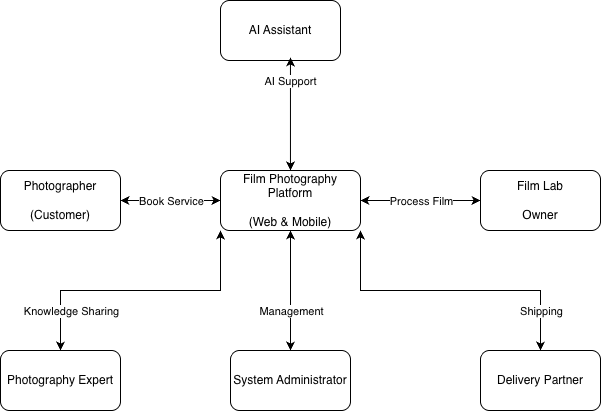
\includegraphics[width=0.90\textwidth]{images/Platform Ecosystem.png}
		\caption{Platform Ecosystem of the Proposed Solution}
		\label{fig:platform_ecosystem}
	\end{figure}
	
	\clearpage
	
	%%%%%%%%%%%%%%%%%%%%%%%%%%%%%%%%%%%%%%%%%%%%%%%%%%%%%%%%%%%%
	
	\subsection{System Roles}
	
	\subsubsection{Photographer}
	
	Photographers register accounts, search Film Labs, place service orders, request pickup services, make online payments, download digital scans, organize Digital Film Archives, submit reviews, and communicate with the AI Assistant.
	
	\subsubsection{Film Lab Owner}
	
	Film Lab Owners manage laboratory information, configure service packages, receive customer orders, update processing status, upload digital scan files, monitor revenue, and generate business reports.
	
	\subsubsection{Photography Expert}
	
	Photography Experts publish educational articles, review cameras and films, organize workshops, answer community questions, and continuously contribute knowledge to the AI knowledge base.
	
	\subsubsection{Delivery Partner}
	
	Delivery Partners receive pickup requests, collect film rolls, transport them to Film Labs, return processed films to customers, and update delivery status.
	
	\subsubsection{System Administrator}
	
	System Administrators manage users, approve Film Labs, moderate community content, monitor payments, resolve disputes, and maintain overall platform performance.
	
	\subsubsection{AI Assistant}
	
	The AI Assistant recommends suitable Film Labs, suggests appropriate film types, performs semantic search, answers photography questions, analyzes scan quality, and provides personalized assistance.
	
	%%%%%%%%%%%%%%%%%%%%%%%%%%%%%%%%%%%%%%%%%%%%%%%%%%%%%%%%%%%%
	
	\subsection{Research-Based Learning (RBL)}
	
	This project follows the Research-Based Learning (RBL) approach by integrating Artificial Intelligence technologies into software engineering.
	
	The major research topics include:
	
	\begin{itemize}
		\item Recommendation Systems
		\item Computer Vision
		\item Semantic Search
		\item Knowledge Graph
		\item Retrieval-Augmented Generation (RAG)
		\item Large Language Models (LLMs)
		\item Community-based Recommendation
		\item Digital Asset Management
	\end{itemize}
	
	Recommendation Systems provide personalized Film Lab suggestions.
	
	Computer Vision evaluates image scan quality.
	
	Semantic Search improves information retrieval.
	
	Knowledge Graph organizes photography knowledge.
	
	RAG combines external knowledge with Large Language Models to improve AI responses.
	
	\begin{figure}[H]
		\centering
		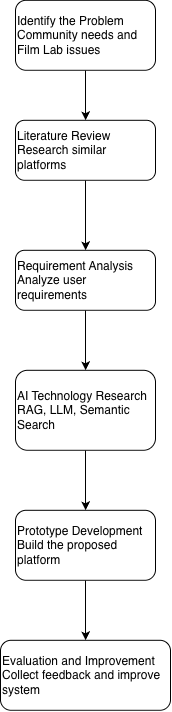
\includegraphics[height=0.65\textheight,keepaspectratio]{images/Research-Based Learning.png}
		\caption{Research-Based Learning Process}
		\label{fig:rbl}
	\end{figure}
	
	\clearpage
	
	%%%%%%%%%%%%%%%%%%%%%%%%%%%%%%%%%%%%%%%%%%%%%%%%%%%%%%%%%%%%
	
	\subsection{Research Approach}
	
	The research methodology consists of the following stages.
	
	\begin{enumerate}
		\item Literature Review
		\item Data Collection
		\item AI Model Design
		\item Experimental Evaluation
		\item Performance Comparison
		\item Model Selection
		\item System Integration
		\item Testing and Validation
	\end{enumerate}
	
	This research process ensures that the selected AI models achieve high recommendation accuracy, reliable image quality assessment, intelligent semantic retrieval, and effective conversational support.
	
	\begin{figure}[H]
		\centering
		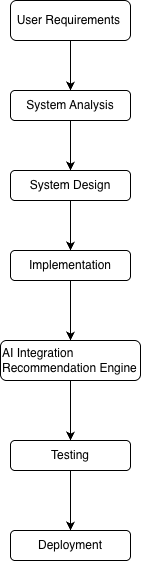
\includegraphics[height=0.65\textheight,keepaspectratio]{images/Research Approach.png}
		\caption{Research Approach of the Proposed System}
		\label{fig:research_approach}
	\end{figure}
	
\end{document}